\documentclass[conference]{IEEEtran}
\usepackage[T1]{fontenc}
\usepackage[utf8]{inputenc}
\usepackage{amsmath,amssymb,graphicx,booktabs,cite,url,etoolbox}
\usepackage[hidelinks]{hyperref}
\patchcmd{\abstract}{---}{.\ }{}{\errmessage{Abstract separator patch failed}}
\patchcmd{\IEEEkeywords}{---}{.\ }{}{\errmessage{Keyword separator patch failed}}
\title{Depth, Compliance, and Verification in a Spatial Cantilever Truss}
\author{Anonymous review draft}
\begin{document}
\maketitle
\begin{abstract}
Changing the depth of a truss changes both its mechanical response and the amount of material required by its members. We examine this tradeoff in a reproducible linear elastic model with 20 nodes and 60 axial bars. Three depths are compared at fixed span, width, bar area, elastic modulus, and total load. Increasing depth from 0.04 to 0.36~m reduces the computed mean tip deflection from 8.779 to 0.1199~mm while increasing member volume from 2.309 to 3.101 litres. An independent implementation reconstructs the stiffness matrix, member forces, reactions, and strain energy from saved geometry. All three cases satisfy force and energy checks at a relative tolerance of $10^{-7}$ and reproduce the saved displacements. The result is a computational case study, not a new structural theory or a construction design. Its verification concerns a linear pin-jointed model and does not cover buckling, connection behavior, or large-displacement response.
\end{abstract}
\begin{IEEEkeywords}
spatial truss, linear elasticity, reproducibility, numerical verification
\end{IEEEkeywords}
\section{Introduction}
A small numerical residual can coexist with an unsuitable physical model. Reproducible research must expose its assumptions, preserve the computed data, and support checks independent of the accompanying narrative.

This study examines one concrete question: how does depth change the deflection and material volume of a specified spatial cantilever truss? The calculation follows the established direct stiffness method, in which transformed member relations are assembled and the free degrees of freedom are solved subject to support constraints~\cite{purdue}. The contribution is a reproducible comparison and a separate verification implementation. The three evaluated configurations do not establish an optimum over possible topologies or dimensions.

\section{Methods}
\subsection{Geometry, material, and loading}
Five equally spaced cross-sections span $x=0$ to $2$~m in increments of $0.5$~m. Each contains four nodes at $(x,\pm0.1,\pm h/2)$, giving a span of 2~m and a width of 0.2~m. The saved connectivity contains 60 unique undirected bars. It is held fixed while the depth $h$ takes the values 0.04, 0.12, and 0.36~m. Coordinates and the complete edge list are provided in the companion data; the edge list, rather than a verbal triangulation rule, defines the reproduced topology.

Every bar has area $A=10^{-4}$~m$^2$ and modulus $E=210$~GPa. All 12 translational degrees of freedom at $x=0$ are fixed. A downward force of 25~N is applied to each of the four nodes at $x=2$~m. The total applied force is therefore 100~N. Self-weight, rotational degrees of freedom, and member bending stiffness are omitted. Nodes are ideal pin joints, and all calculations use the undeformed geometry.

\subsection{Stiffness and response}
For a member joining nodes $i$ and $j$, let $L_e$ be its length and let $n_e=(x_j-x_i)/L_e$ be its unit direction. Its global translational stiffness is
\begin{equation}
 K_e=\frac{EA}{L_e}
 \begin{bmatrix} n_en_e^T&-n_en_e^T\\-n_en_e^T&n_en_e^T\end{bmatrix}.
 \label{eq:member}
\end{equation}
After assembly, zero prescribed support displacement gives $K_{ff}u_f=f_f$. The independent implementation uses NumPy's dense linear solver~\cite{numpy}. The 48 free degrees of freedom make a dense representation adequate for this verification; no performance comparison is claimed. The smallest computed eigenvalue of each reduced matrix is positive, providing a numerical check against an unconstrained mechanism in these instances.

Tip deflection is the magnitude of the mean vertical displacement of the four loaded nodes. Material volume is $V=A\sum_e L_e$. Volume counts the ideal bars only, excluding joints, overlapping material, and fabrication details. Because the topology is fixed, changing depth also changes diagonal member lengths and hence $V$.

\subsection{Independent verification}
The verification program reads the saved coordinates and connectivity, rebuilds $K$, and solves the constrained system. It then reconstructs each axial extension directly from the displacement difference,
\begin{equation}
 d_e=n_e^T(u_j-u_i),\qquad N_e=\frac{EA}{L_e}d_e,
 \label{eq:force}
\end{equation}
and adds the corresponding force vectors to the two end nodes. The free-node residual is normalized by $\|f\|_2$. The total reaction-plus-load imbalance is normalized by the same quantity. These checks use member-force accumulation, rather than only multiplying the assembled matrix by the solution.

The member energy and load work are
\begin{equation}
 U=\frac12\sum_e\frac{EA}{L_e}d_e^2,
 \qquad W=f^Tu.
 \label{eq:energy}
\end{equation}
The program requires positive $U$ and relative discrepancy $|2U-W|/|W|<10^{-7}$. It also checks the expected linear scaling under doubled load and doubled stiffness. Saved tip displacements are reproduced within $10^{-10}$~m. These tolerances are verification criteria for this small numerical study, not engineering acceptance limits.

\section{Results}
Table~\ref{tab:results} reports the three computed cases. The deeper configurations require more bar material and produce substantially less vertical deflection under the same load. From the shallowest to the deepest case, deflection falls by a factor of about 73.2 while volume increases by about 34.3\%. Figure~\ref{fig:tradeoff} presents the same comparison. The logarithmic deflection axis makes both decreases visible; it does not imply a fitted power law.

\begin{table}[t]
\caption{Response at 100 N over a span $L=2$ m}
\label{tab:results}
\centering
\begin{tabular}{rrrr}
\toprule
$h$ (m)&$|u_{\rm tip}|$ (mm)&$V$ (litres)&$|u_{\rm tip}|/L$\\
\midrule
0.04&8.779&2.309&$4.390\times10^{-3}$\\
0.12&0.9838&2.447&$4.919\times10^{-4}$\\
0.36&0.1199&3.101&$5.994\times10^{-5}$\\
\bottomrule
\end{tabular}
\end{table}

\begin{figure}[t]
\centering
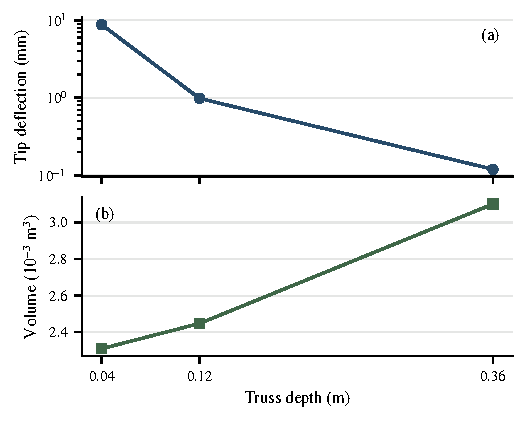
\includegraphics[width=\columnwidth]{depth-tradeoff.pdf}
\caption{Effect of depth for the fixed 20-node, 60-bar topology: (a) mean loaded-end deflection and (b) ideal member volume. Each marker is a separately verified configuration at 100 N. Connecting lines guide the eye; intermediate configurations were not evaluated.}
\label{fig:tradeoff}
\end{figure}

All three cases passed the independent force-balance, energy, displacement-reproduction, and linear-scaling checks. A separately saved check for the medium-depth case reported a free-force residual of $1.34\times10^{-12}$ and a total force-balance residual of $1.34\times10^{-12}$. Its reconstructed energy was approximately 0.04918768~J, compared with $W\approx0.09837536$~J, consistent with Eq.~\eqref{eq:energy}. These figures describe that saved calculation; different floating-point accumulation orders can change the final few digits.

\section{Discussion and Limitations}
The trend is compatible with the geometry of a deeper triangulated structure resisting transverse loading more effectively through axial forces. However, three depths and one connectivity do not establish a general scaling law, an optimal design, or a ranking across other topologies. The numerical experiment isolates a specific geometric change while holding the other stated parameters fixed.

The corrected load also matters. An earlier run at 10 kN produced approximately 0.878~m of shallow-case tip deflection, about 44\% of the span. Interpreting that result as a physically credible small-displacement response would be unjustified. Reducing the load to 100~N reduces the corresponding ratio to about 0.439\%, but a small global ratio alone does not validate every modeling assumption. The largest computed axial strain in the corrected cases is approximately $1.13\times10^{-4}$; constitutive and stability questions still require their own justification.

The independent program checks internal consistency and reproduces the stated model. It is not a mesh-convergence study, experimental validation, or an independent implementation of a different physical theory. Member buckling, geometric stiffness, yielding, imperfection sensitivity, joint flexibility, and connection strength are outside the calculation. A structurally useful design would require these effects and appropriate loading and acceptance criteria. No such design claim is made here.

This deterministic study does not estimate statistical uncertainty or establish solver performance. Numerical precision is distinct from physical validity.

\section{Conclusion}
For the specified axial-bar model, increasing depth from 0.04 to 0.36~m substantially reduces computed deflection at a moderate increase in ideal member volume. The saved results can be reproduced and checked through independent stiffness assembly and direct member-force and energy reconstruction. The useful outcome is an inspectable calculation with a clear boundary between numerical consistency and physical validation.

\section*{Reproducibility and Authorship}
The accompanying files include the original corrected data, the exact geometry and edge lists, the verification and figure-generation script, its execution record, this source, the bibliography, and the compiled PDF. The deterministic verification uses Python 3.13 and NumPy 2.2.6 in an isolated CPU container. This AI-assisted anonymous draft requires review by its responsible authors before submission.

\bibliographystyle{IEEEtran}
\bibliography{references}
\end{document}
